% Chapter 7

\begin{savequote}[45mm]
Modified\ldots
\qauthor{Ancient proverb}
\end{savequote}

\chapter{Application: Modified SFC} % Main chapter title

\label{Chapter7} % For referencing this chapter elsewhere, use \ref{Chapter7}

\section{Introduction}

In the previous chapter the SFC×GC was run with neat carbon dioxide as mobile
phase for the SFC dimension. Carbon dioxide as a mobile phase is compatible with
an FID detector: under the conditions found in the hydrogen-rich portion flame
the carbon dioxide cannot be reduced to methane, the first step in the process
that produces the ions that gives the FID it's name. But most modern SFC
development involves the use of modifiers and additives. Modifiers are added to
the carbon dioxide to manipulate the solubility of the analytes in the mobile
phase, in exactly the same way that mixtures of solvents are used in, say,
gradient elution in HPLC. Additives are added in small amounts, and manipulate
the interaction of the analyte with the mobile phase. These modifiers are
usually organic compounds, and they produce ions in a flame. Because the
modifiers are present in much higher quantities than the analytes, they will
produce many more ions in an FID than any ions from the analyte, and therefore
the analyte signal will be swamped by the modifier signal. The introduction of
the use of organic additives and modifiers to the carbon dioxide mobile phase
has therefore made modern SFC incompatible with flame ionization as a detection
method.

Therefore, most modern SFC chromatographs use optical detectors, most commonly
UV spectrophotometry. But selecting UV spectrophotometry as a detector for SFC
imposes other limitations: only modifiers that don't absorb UV radiation can be
used, and of course only analytes with chromophores can be detected. If only
there were a way to separate the the modifiers from the analytes before
detections \ldots

But a mixture of analytes and volatile organic modifiers can be readily
separated using gas chromatography. If fractions

\section[SFC×GC ]{SFC×GC using modified}

\subsection{Sample}

The sample was a 1:1 blend of petrodiesel and biodiesel, prepared in the
laboratory. The biodiesel sample was donated by a commercial testing laboratory,
and was produced from palm oil by an anonymous producer. The petrodiesel (Shell
Extra Diesel 500 ppm) was obtained from a commercial filling station.


\subsection{SFC}

The SFC used carbon dioxide at \SI{200}{\bar} inlet pressure and room
temperature as mobile phase. The flow rate is of carbon dioxide at atmospheric
pressure was reportedly \SI{175}{\milli\litre\per\minute}. The carbon dioxide
mobile phase was modified with \SI{5}{\percent} mass fraction of HPLC-grade
methanol (Merck LiChrosolv). The column consisted of five HPLC bare silica
columns (150 mm $\times$ 4.6 mm, 3 $\mu$m particles) (Restek, Pinnacle DB
Silica) connected in series.

\subsection{Modulation}

GC idle temperature:	293.100000 Cdeg
GC purge temperature: 	323.150000 Cdeg
GC sampling temperature: 	233.150000 Cdeg
GC sampling time: 	5
GC load time: 	3
GC vent time: 	1

GC column description:	Rxi-5Sil MS 0.250 mm x 1 m

GC flow rate: 	11.600
Experiment title: 	Polarity mix
Sample name: 	Test Mix A
Analysis type: 	Standard
Concentration: 	5000.000
Operator name: 	DM
Detector sensitivity: 	2.0E-10
FID H2 flow rate: 	50.000
FID Air flow rate: 	300.000
SFC pressure: 	20265000 Pa
SFC dead time: 	720.000 s
%File name: 	C:\SFC-GC\Data\2016_12_08-140548.dat


\subsection{GC}

GC gradient0:
Rate: 	0 $1 s^-1
Final:	233.150000 $1
Time:	0.000 s
GC gradient1:
Rate: 	33 $1 s^-1
Final:	593.150000 $1
Time:	10.000 s


\subsection{Results and discussion}

The chromatogram obtained from this run is shown in Figure \ref{fig:Modifier}

The intention of this chromatographic run was to exlore the 

See Figure \ref{fig:Modifier}

\begin{figure}
	\centering
	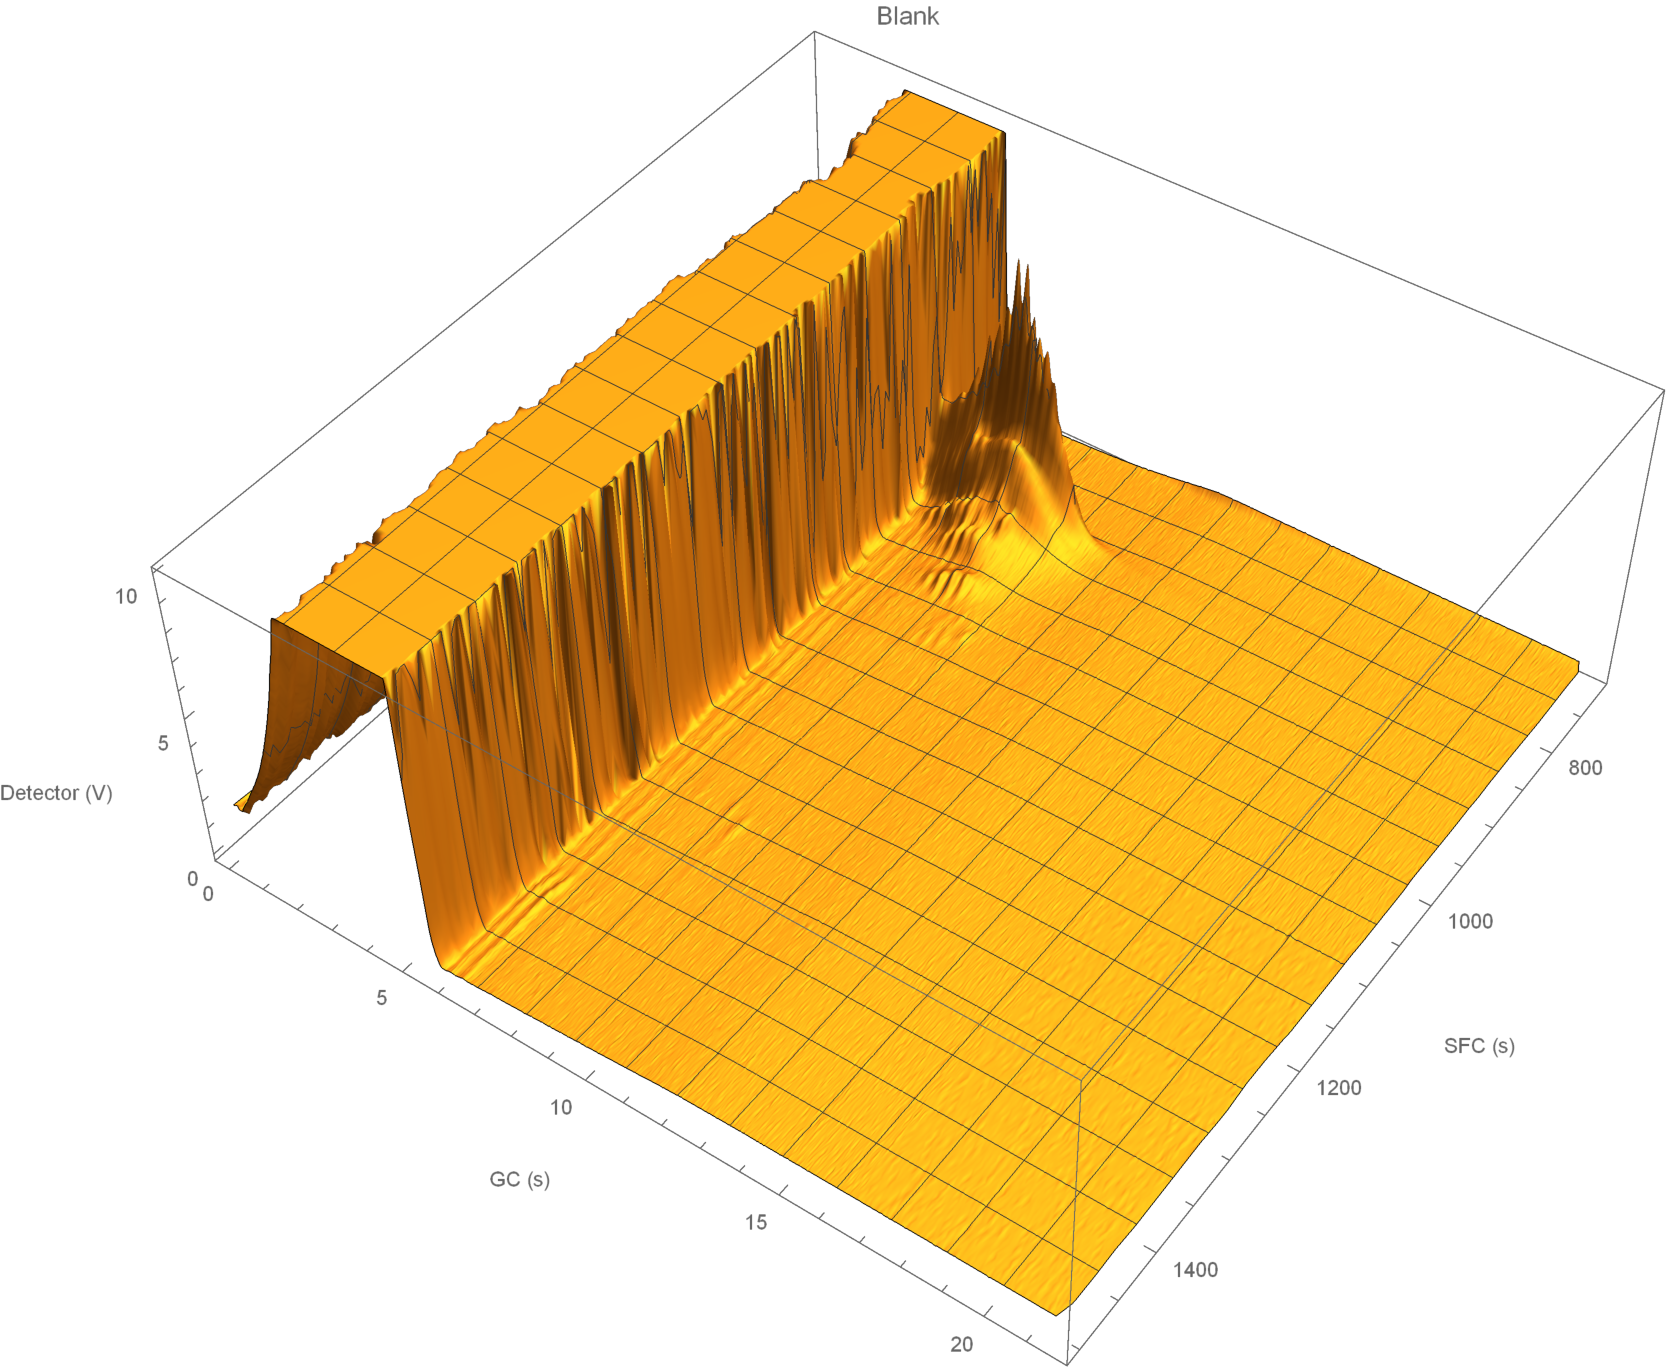
\includegraphics[width=\textwidth]{Figures/Modifier.pdf}
	\decoRule	
	
	\caption[Modifiers in SFC]{The modifiers used in the SFC dimension elutes as a
solvent front on the GC dimension, and does not otherwise affect the separation.}
	
	\label{fig:Modifier} 
\end{figure}

\subsection{Discussion}

